% document configuration
% document class
\documentclass[10pt]{beamer}

% libraries
\usepackage[utf8]{inputenc}

% presentation theme
\usetheme{Madrid}

% colors
\usepackage{xcolor}
\definecolor{forestgreen}{HTML}{1d771d}



% animation of images
\usepackage{animate}

% figure configuration
\usepackage{caption}
\captionsetup[figure]{font=scriptsize, justification=centering}

% break equation
\usepackage{amsmath}

% outile configuration
\setbeamerfont{section in toc}{size=\large}
\setbeamerfont{subsection in toc}{size=\small}
\setbeamertemplate{section in toc}[sections numbered]




% introduction parameters
\title[Article presentation]{title}

\author[J. Charaja and S. Munoz]{Jhon Charaja\inst{1} and Samir Munoz\inst{2}}
\institute[USP]{
	\inst{1} Universidade de São Paulo, Brasil \\
	\inst{2} Universidad de Ingeniería y Tecnología, Perú
}

\date{\today}


\begin{document}
	\frame{\titlepage}
	% methodology
	\section{Methodology}
	
	\begin{frame}
		\frametitle{Sliding mode control with fixed gains}
		%\fboxrule=3pt
		%\fcolorbox{red}{white}{
		
		\begin{minipage}[t]{0.45\textwidth}
			\graphicspath{{images/methodology/SMC/exp1/circular/uncertainty_100_alpha_0/}}
			\centering
			{\large \textbf{factory value ($m_6=m_6$)}} \\
			\vspace{.2cm}
			{\color{blue} \textbf{uncertainty: $0\%$}} \\
			{\color{forestgreen} \textbf{desired pose}: \scalebox{1.5}{$\bullet$}} \\
			{\color{darkyellow}  \textbf{current pose}: \scalebox{1.5}{$\bullet$}} \\			
			
						
			\animategraphics[controls={play}, loop, width=\textwidth]{60}{}{10}{20}
		\end{minipage}
		%}
		\hspace{.08\textwidth}
		%\fcolorbox{black}{white}{
		\begin{minipage}[t]{0.45\textwidth}
			\graphicspath{{images/methodology/SMC/exp1/circular/uncertainty_100_alpha_0/}}
			\centering
			{\large \textbf{new mass value ($m_6=2 m_6$)}}\\
			\vspace{.2cm}
			{\color{blue} \textbf{uncertainty: $100\%$}} \\
			{\color{forestgreen} \textbf{desired pose}: \scalebox{1.5}{$\bullet$}} \\
			{\color{darkyellow}  \textbf{current pose}: \scalebox{1.5}{$\bullet$}} \\	
			
						
			\animategraphics[controls={play}, loop, width=\textwidth]{60}{}{10}{20}
		\end{minipage}
		%}
		\comment{
		\begin{table}
			\caption{trajectory tracking error with L2 norm ($t=500$ s)}
			\centering
			\begin{tabular}{c c c}
			\toprule
			uncertainty & position ($\mathrm{mm}$) & jerk linear ($\mathrm{\frac{mm}{s^3}}$) \\
			\midrule
			0.0 \%  & 0.49 & 0.21 \\ 
			100 \% & 19.7 & 3.04\\
			\bottomrule
			\end{tabular}
		\end{table}		
		}

	\end{frame}

	\begin{frame}
		\frametitle{Sliding mode control with optimization equations}
		
		\fboxrule=3pt
		%\fcolorbox{red}{white}{
		\begin{minipage}[t]{0.45\textwidth}
			\graphicspath{{images/methodology/SMC/exp1/circular/uncertainty_100_alpha_0/}}
			\centering
			{\large \textbf{fixed gains ($m_6=2m_6$)}}
			%\vspace{.2cm}			
			\animategraphics[controls={play}, loop, width=\textwidth]{60}{}{10}{20}
		\end{minipage}
		%}
		\hspace{.08\textwidth}
		%\fcolorbox{black}{white}{
		\begin{minipage}[t]{0.45\textwidth}
			\graphicspath{{images/methodology/SMC/exp1/circular/uncertainty_100_alpha_0.005/}}
			\centering
			{\large \textbf{optimized gains ($m_6=2 m_6$)}}
			%\vspace{.2cm}
			\animategraphics[controls={play}, loop, width=\textwidth]{60}{}{10}{20}
		\end{minipage}
		%}
		
		\begin{table}
			\caption{trajectory tracking error with L2 norm ($t=500$ s)}
			\centering
			\begin{tabular}{c c c c c}
			\toprule
			gain type & position ($\mathrm{mm}$) & orientation ($^\circ$) & jerk linear ($\mathrm{\frac{mm}{s^3}}$) & jerk angular \\
			\midrule
			fixed  & 19.7 & 50.3 & 3.04 & 0 \\ 
			optimized & 7.28 & 4.5 & 0.98 & 0  \\
			\bottomrule
			\end{tabular}
		\end{table}		
	\end{frame}	
	
	\begin{frame}
		\frametitle{Sliding mode control}
		\graphicspath{{images/methodology/SMC/exp1/circular/uncertainty_100_alpha_0.005/}}
		\begin{figure}
			\centering
			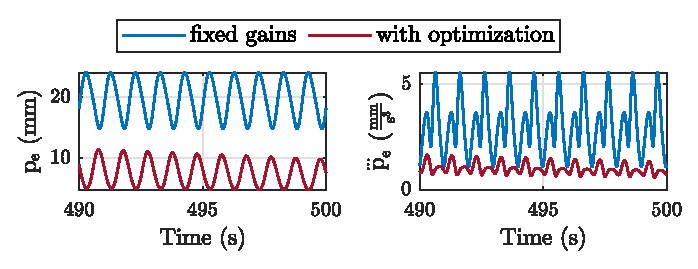
\includegraphics{pe_cartesian.eps}
		\end{figure}

		\begin{table}
			\caption{trajectory tracking error with L2 norm ($t=500$ s)}
			\centering
			\begin{tabular}{c c c c c}
			\toprule
			gain & position ($\mathrm{mm}$) & orientation ($^\circ$) & jerk linear ($\mathrm{\frac{mm}{s^3}}$) & jerk angular \\
			\midrule
			fixed  & 19.7 & 50.3 & 3.04 & 0 \\ 
			optimized & 7.28 & 4.5 & 0.98 & 0  \\
			\bottomrule
			\end{tabular}
		\end{table}		
	\end{frame}	



	\begin{frame}
		\frametitle{Proportional-Derivative control with fixed gains}
		%\fboxrule=3pt
		%\fcolorbox{red}{white}{
		
		\begin{minipage}[t]{0.45\textwidth}
			\graphicspath{{images/methodology/SMC/exp1/circular/uncertainty_100_alpha_0/}}
			\centering
			{\large \textbf{factory value ($m_6=m_6$)}} \\
			\vspace{.2cm}
			{\color{blue} \textbf{uncertainty: $0\%$}} \\
			{\color{forestgreen} \textbf{desired pose}: \scalebox{1.5}{$\bullet$}} \\
			{\color{darkyellow}  \textbf{current pose}: \scalebox{1.5}{$\bullet$}} \\			
			
						
			\animategraphics[controls={play}, loop, width=\textwidth]{60}{}{10}{20}
		\end{minipage}
		%}
		\hspace{.08\textwidth}
		%\fcolorbox{black}{white}{
		\begin{minipage}[t]{0.45\textwidth}
			\graphicspath{{images/methodology/SMC/exp1/circular/uncertainty_100_alpha_0/}}
			\centering
			{\large \textbf{new mass value ($m_6=2 m_6$)}}\\
			\vspace{.2cm}
			{\color{blue} \textbf{uncertainty: $100\%$}} \\
			{\color{forestgreen} \textbf{desired pose}: \scalebox{1.5}{$\bullet$}} \\
			{\color{darkyellow}  \textbf{current pose}: \scalebox{1.5}{$\bullet$}} \\	
			
						
			\animategraphics[controls={play}, loop, width=\textwidth]{60}{}{10}{20}
		\end{minipage}
		%}
		\comment{
		\begin{table}
			\caption{trajectory tracking error with L2 norm ($t=500$ s)}
			\centering
			\begin{tabular}{c c c}
			\toprule
			uncertainty & position ($\mathrm{mm}$) & jerk linear ($\mathrm{\frac{mm}{s^3}}$) \\
			\midrule
			0.0 \%  & 0.49 & 0.21 \\ 
			100 \% & 19.7 & 3.04\\
			\bottomrule
			\end{tabular}
		\end{table}		
		}

	\end{frame}

	
	\begin{frame}
		\frametitle{Proportional-Derivative control with optimization equations}
		
		\fboxrule=3pt
		%\fcolorbox{red}{white}{
		\begin{minipage}[t]{0.45\textwidth}
			\graphicspath{{images/methodology/SMC/exp1/circular/uncertainty_100_alpha_0/}}
			\centering
			{\large \textbf{fixed gains ($m_6=2m_6$)}}
			%\vspace{.2cm}			
			\animategraphics[controls={play}, loop, width=\textwidth]{60}{}{10}{20}
		\end{minipage}
		%}
		\hspace{.08\textwidth}
		%\fcolorbox{black}{white}{
		\begin{minipage}[t]{0.45\textwidth}
			\graphicspath{{images/methodology/SMC/exp1/circular/uncertainty_100_alpha_0.005/}}
			\centering
			{\large \textbf{optimized gains ($m_6=2 m_6$)}}
			%\vspace{.2cm}
			\animategraphics[controls={play}, loop, width=\textwidth]{60}{}{10}{20}
		\end{minipage}
		%}
		
		\begin{table}
			\caption{trajectory tracking error with L2 norm ($t=500$ s)}
			\centering
			\begin{tabular}{c c c c c}
			\toprule
			gain & position ($\mathrm{mm}$) & orientation ($^\circ$) & jerk linear ($\mathrm{\frac{mm}{s^3}}$) & jerk angular \\
			\midrule
			fixed  & 49.2 & 27.9 & 1.34 & 0 \\ 
			optimized & 20.5 & 8.12 & 0.85 & 0  \\
			\bottomrule
			\end{tabular}
		\end{table}			
	\end{frame}		

	\begin{frame}
		\frametitle{Proportional-Derivative control}
		\graphicspath{{images/methodology/PD/exp1/circular/uncertainty_100_alpha_0.005/}}
		\begin{figure}
			\centering
			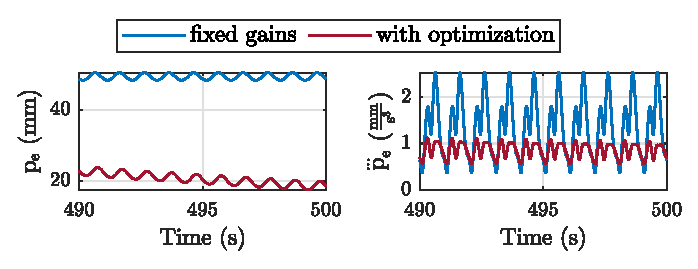
\includegraphics{pe_cartesian.eps}
		\end{figure}

		\begin{table}
			\caption{trajectory tracking error with L2 norm ($t=500$ s)}
			\centering
			\begin{tabular}{c c c c c}
			\toprule
			gain & position ($\mathrm{mm}$) & orientation ($^\circ$) & jerk linear ($\mathrm{\frac{mm}{s^3}}$) & jerk angular \\
			\midrule
			fixed  & 49.2 & 27.9 & 1.34 & 0 \\ 
			optimized & 18.6 & 7.5 & 0.83 & 0  \\
			\bottomrule
			\end{tabular}
		\end{table}		
	\end{frame}	
	
	\begin{frame}
		\renewcommand{\arraystretch}{1.25}
		\begin{table}
			\caption{trajectory tracking error with L2 norm ($t=500$ s)}
			\centering			
			\begin{tabularx}{0.99\textwidth}{
			>{\centering\arraybackslash}X
			>{\centering\arraybackslash}X
			>{\centering\arraybackslash}X
			>{\centering\arraybackslash}X
			>{\centering\arraybackslash}X
			>{\centering\arraybackslash}X}
			\toprule
			control method & 
			uncertainty ($\%$) & 
			position ($\mathrm{mm}$) & 
			orientation ($^\circ$) & 
			jerk linear ($\mathrm{\frac{mm}{s^3}}$) & 
			jerk angular ($\mathrm{\frac{^\circ}{s^3}}$) \\
			\midrule
			\multirow{3}{*}{PD} 
			& $25$ & $19.7$ & $7.81$ & $0.45$  &  \\
			& $50$ & $23.8$ & $8.94$ & $0.67$ & \\
			& $75$ & $21.7$ & $8.31$ & $0.77$ & \\
			& $100$ &$18.57$ & $7.52$ & $0.83$ & \\						
			\midrule
			\multirow{3}{*}{SMC} 
			& $25$ & $7.46$ & $3.02$ & $0.66$ &  \\
			& $50$ & $8.21$ & $3.76$ & $0.91$ & \\
			& $75$ & $8.06$ & $4.32$ & $0.98$ & \\
			& $100$ & $7.23$ & $4.48$ & $0.91$ & \\	
			\bottomrule			
			\end{tabularx}
		\end{table}
	

	\end{frame}
	
\end{document}